
\documentclass{article}

\usepackage{verbatim}
\usepackage{cite}
\usepackage{parskip}
\usepackage{longtable}
\usepackage{listings}
\usepackage{graphicx}
\usepackage[margin=1in]{geometry}
\begin{document}

\title{An atempt at Just-In-Time compilation\\of haskell using PyPy and GHC}
\author{Knut Halvor Skrede}
\maketitle

\begin{abstract}
Abstract
\end{abstract}

\clearpage

\tableofcontents

\clearpage

\setlength\LTleft{0pt}
\setlength\LTright{0pt}

% Introduction


\chapter{Introduction}

This chapter discusses the motivation behind the project and 
presents a description of the project and of the work done. It 
is concluded by introducing the remaining chapters.

\section{Motivation and project description}

The project aims to investigate the feasibility of JIT (Just-in-time) 
compilation of a strongly-typed purely-functional language. Since
programs written in such a language can be heavily optimized at 
compile time, it is uncertain whether such programs can benefit from
JIT compilation. However, a JIT compiler has a lot more information to
work with than a static compiler. 

To test this, the techniques 
used by the PyPy (Python in Python) project are applied to the Haskell 
programming language. By implementing the back-end for a Haskell compiler 
in RPython (restricted Python), and using GHC (the Glasgow Haskell Compiler) 
as a front-end, a full Haskell JIT compiler can be implemented. An 
interpreter for a language very similar to the intermediate language used
by GHC was already implemented, and this is the base for this project.
Although it is already possible to have JIT compilation with GHC through
its LLVM back-end, the PyPy approach will interpret code at a much higher level.

We focus on implementing a serializer from Haskell to an intermediate
format using GHC, and a deserializer from that format to the interpreter. The 
interpreter is for a language similar to Core (the intermediate format used by GHC.)
By implementing some simple programs in Haskell, and running them through our 
compilation system, 
we hope to show that the methods of the PyPy project can be successfully applied 
to pure functional languages such as Haskell.

\section{Contributions}
The contributions of this thesis is a description of Haskell-Python (an
interpreter for Core' (a lambda-calculus inspired by Haskell)), and a system for
translating Haskell programs into Core'. In addition to this, the paper 
presents a description of the full compilation system in its current state,
and a plan for the future development of the system based on the 
successes and failures so far.

Following is a listing describing how the work in this project has been
partitioned.

The following work had already been done:
\begin{itemize}

\item The Haskell-Python\cite{haskellpython} interpreter was written.

\end{itemize}

These parts were the result of an earlier stage of the project:
\begin{itemize}

\item An investigation into the use of GHC as a front-end for the compiler.
This resulted in the JSCore intermediate language, but was unsuccessful
at creating JSCore files from the GHC Haskell libraries.

\item A parser for the JSCore language was implemented; however, this 
parser was only successful for a very small subset of the JSCore language.

\item A simple system for testing functionality was implemented.

\end{itemize}

For this project, the following has been done:
\begin{itemize}

\item Another attempt was given at the creation of JSCore for the GHC 
Haskell libraries, but was still unsuccessful. The reason for this being
bugs in GHC. Specifically, bugs in the code that dumps the External-Core
files.

\item Various Haskell values and functions have been implemented at a higher
level. Due to the fact that we could not successfully create intermediate
files for the Haskell
libraries we had to implement the functionality at a higher level, i.e. 
Python.

\item Based on the gained understanding of the Core language from the
previously mentioned work, the parser has been improved. The result of 
the improvements to the parser, with the implementation of the libraries,
has resulted in the successful execution of some less trivial programs,
such as a naive recursive implementation of fibonacci.

\end{itemize}

In addition to this, some work has been done in parallell by E.W.Thomassen,
most notably:
\begin{itemize}

\item Refactoring of the code written previously, in order to make it better 
match other PyPy projects.

\item Rewriting the Python code into RPython, such that it can be translated by
the PyPy toolchain.

\item He has also changed quite a bit of the functionality for the better,
and details of this work can be found in his report.

\end{itemize}

% Write about the use-cases of laguages like Haskell, and the benefits of 
% Jit compilation

% + Research blahblah... Just to see if it works well.

% Structure of the paper. TODO
\section{Structure of the paper}
In chapter \ref{chap:back} some background information is presented, including 
some terms and concepts. 
%
A description of the 
Haskell-Python interpreter is given in chapter \ref{chap:hs}.
%
Chapter \ref{chap:rewrite} goes into detail regarding the intermediate 
languages, and the mapping between them.
%
%In chapter \ref{chap:prims} the Haskell libraries and necessary primitives
%are discussed.
%
%Chapter \ref{chap:pipe} describes the entire pipeline of the compilation system 
%at a high level.
%
%Chapter \ref{chap:test} describes the test-system used.
%
Chapter \ref{chap:impl} contains a description of the compilation system.
%
In chapter \ref{chap:similar} a brief discussion of similar work is presented.
%
Chapter \ref{chap:bench} presents some preliminary benchmark results.
%
Everything is concluded in chapter \ref{chap:conc}, which discusses 
the results and future work.


% PYPY

\section{PyPy}

\subsection{A quick overview}

The PyPy project is basically two things:

\begin{enumerate}

\item The RPython toolchain; a set of compiler tools for programs written in 
RPython.

\item An implementation of Python using these tools.

\end{enumerate}

In this paper PyPy refers to former.

The basic concept of PyPy is to use a high-level language to allow for rapid
development of interpreters for a variety of platforms. By implementing a compiler
for RPython, interpreters for other languages can be written in RPython and 
compiled to any platform supported by the PyPy toolchain.

\subsection{RPython}

RPython is a restricted proper subset of Python, this enables easy analysis 
as well as efficient compilation.

\subsection{Translation toolchain}


\subsection{Just-in-time compilation}

The reason why PyPy is able to compete with other language implementations
on speed is it's tracing, or rather meta-tracing, JIT. The JIT is implemented
for RPython, but through a set of compiler hints, it is able to trace the 
execution of the application interpreted by the RPython program.

An introduction to virtual machine (VM) construction with python \cite{pypy}.



% Haskell

\section{GHC}

\emph{Haskell} is a \emph{strongly-typed non-strict purely-functional} programming language, it will not be
described in detail here, since Haskell is not the language we focus on. See \cite{hudak1992report}
for an introduction to Haskell. 

Core is an intermediate language used by the Glasgow Haskell Compiler\cite{ghc},
and it is this language we wish to interpret. Core is a desugared version of Haskell, things like pattern matching
and list comprehensions are transformed out to simpler constructs.\cite{jones1994compilation}

\subsection{Compilation by transformation}

GHC uses a compilation idiom called \emph{compilation by transformation}. The idea is to repeatedly perform 
correctness-preserving transformations to the program. Ideally, these transformations will result
in a semantically equal program that executes more quickly or in less space. Such transformations seem
to fall into two categories:

\begin{itemize} 
\item{\emph{Glamorous transformations}} are global, sophisticated, intellectually satisfying transformations,
sometimes guided by some interesting kind of analyzis.
\item{\emph{Humble transformations}} are small, simple, local transformations. Individually they look very trivial.
\end{itemize}

In the Glasgow Haskell Compiler, all humble transformations are done by the \emph{simplifier}. 
\cite{jones1994compilation} The simplifier repeatedly performs transformations on the Core language.


\subsection{The GHC API and usage}

...




% Core


\section{External-core}


% New

The Core language is an intermediate language used by GHC. It is the internal
program representation in the compilers simplification phase. External-core
is an external representation of Core generated by using a compiler flag. 
By using external-core, one
may implement just parts of a Haskell compiler, using the remaining parts from
GHC. For this project, GHC is used to generate external-core. This way, desugaring,
type checking, pattern matching and overloading is performed. The remaing task
is then to interpret the external-core representation. \cite{tolmach2010ghc}

Without using GHC to produce external-core, linking code into GHC would be an 
optional way of achieving this, which would be a difficult and large task.
Or, the GHC API could be used to do the same task more cleanly. \cite{tolmach2010ghc}

The initial starting point of this project was to use the GHC API, the reason
was that external-core is not fully parenthesized and more tricky to parse. Thus,
generating a fully parenthesized and more machine-readable format would make sense.
However, it turened out that this too was a complicated task. As the internal
core datatypes of GHC does not match the description of external-core. The choice was
then made to use GHC-generated external-core as the base for creating a new intermediate
format that could be easily generated using available packages for manipulating
external-core.


% Old

%The Core language is the internal program representation used by GHC. In Core,
%all syntactic sugar is removed, type checking is performed, pattern matching is
%translated into case-expressions (each of witch performs only a single level of
%matching) and overloading is resolved.\cite{jones1992implementing} Following
%is a description of external-core as presented by \cite{tolmach2010ghc}.

\clearpage

\subsection{External-core language definition}

The following semantics is used to define the Core grammar, 
as seen in \cite{tolmach2010ghc}:

\begin{longtable}{ l c l }

$[$ pat $]$		& :	& optional			\\
$\{$ pat $\}$		& :	& zero or more repetitions	\\
$\{$ pat $\}^{+}$	& :	& one or more repetitions	\\
$pat_{1}|pat_{2}$	& :	& choice			\\

\end{longtable}

\begin{scriptsize}
\begin{longtable}{ r c l r }


\\[0.01in]

\multicolumn{4}{l}{Module}			 \\
\\[0.01in]
$module$	& $ \rightarrow $ 	& \%module $mident$ $\{$ $tdefg$ ; $\}$ $\{$ $vdefg$ ; $\}$				&			\\
\\[0.01in]

\multicolumn{4}{l}{Type defn.}			 \\
\\[0.01in]
$tdefg$ 	& $ \rightarrow $	& \%data $qtycon$ $\{$ $tbind$ $\}$  = $\{$ $[$ $cdef$ $\{$ ; $cdef$ $\}$ $]$ $\}$	& algebraic type	\\
		& $ | $			& \%newtype $qtycon$ $qtycon$ $\{ tbind \}$ = $ty$					& newtype		\\
\\[0.01in]

\multicolumn{4}{l}{Constr. defn.}			 \\
\\[0.01in]
$cdef$		& $ \rightarrow $	& $qdcon$ $\{$ @ $tbind$ $\}$ $\{$ $aty$ $\}^{+}$ 					& 			\\
\\[0.01in]

\multicolumn{4}{l}{Value defn.}			 \\
\\[0.01in]
$vdefg$		& $ \rightarrow $	& \%rec $\{$ $vdef$ $\{$ ; $vdef$ $\}$ $\}$						& recursive		\\
		& $ | $			& $vdef$										& non-recursive		\\
$vdef$ 		& $ \rightarrow $	& $qvar$ :: $ty$ = $exp$								& 			\\
\\[0.01in]

\multicolumn{4}{l}{Atomic expr.}			 \\
\\[0.01in]
$aexp$		& $ \rightarrow $	& $qvar$										& variable		\\
		& $ | $			& $qdcon$										& data constructor	\\
		& $ | $			& $lit$											& literal		\\
		& $ | $			& ( $exp$ ) 										& nested expr.		\\
\\[0.01in]

\multicolumn{4}{l}{Expression}			 \\
\\[0.01in]
$exp$		& $ \rightarrow $	& $aexp$										& atomic expr.		\\
		& $ | $			& $aexp$ $\{$ $arg$ $\}^{+}$ 								& application		\\
		& $ | $			& $\backslash$ $\{$ $binder$ $\}$ -$>$ $exp$						& abstraction		\\
		& $ | $			& \%let	$vdefg$ \%in $exp$								& local definition	\\
		& $ | $			& \%case ( $aty$ ) $exp$ \%of $vbind$ $\{$ $alt$ $\{$ ; $alt$ $\}$ $\}$			& case expr.		\\
		& $ | $			& \%cast $exp$ $aty$									& type coercion		\\
		& $ | $			& \%note "  $\{$ $char$ $\}$ " $exp$							& expression note	\\
		& $ | $			& \%external ccal " $\{$ $char$ $\}$ " $aty$						& external reference	\\
		& $ | $			& \%dynexternal ccal $aty$								& external reference (dynamic)	\\
		& $ | $			& \%label " $\{$ $char$ $\}$ "								& external label	\\
\\[0.01in]

\multicolumn{4}{l}{Argument}			 \\
\\[0.01in]
$arg$		& $ \rightarrow $	& @ $aty$										& type argument		\\
		& $ | $			& $aexp$										& value argument	\\
\\[0.01in]

\multicolumn{4}{l}{Case alt}			 \\
\\[0.01in]
$alt$		& $ \rightarrow $	& $qdcon$ $\{$ @ $tbind$ $\}$ $\{$ $vbind$ $\}$ -$>$ $exp$				& constructor alternative \\
		& $ | $			& $lit$ -$>$ $exp$									& literal alternative 	\\
		& $ | $			& \%\_ -$>$ $exp$									& default alternative	\\
\\[0.01in]

\multicolumn{4}{l}{Binder}			 \\
\\[0.01in]
$binder$	& $ \rightarrow $	& @ $tbind$										& type binder		\\
		& $ | $			& $vbind$										& value binder		\\
\\[0.01in]

\multicolumn{4}{l}{Type binder}			 \\
\\[0.01in]
$tbind$		& $ \rightarrow $	& $tyvar$										& implicit of kind * 	\\
		& $ | $			& ( $tyvar$ :: $kind$ )									& explicitly kinded	\\
\\[0.01in]

\multicolumn{4}{l}{Value binder}			 \\
\\[0.01in]
$vbind$		& $ \rightarrow $	& ( $var$ :: $ty$ )									& \\
\\[0.01in]

\multicolumn{4}{l}{Literal}			 \\
\\[0.01in]
$lit$		& $ \rightarrow $	& ( $[$-$]$ $\{$ $digit$ $\}^{+}$ :: $ty$ )						& integer 		\\ 
		& $ | $			& ( $[$-$]$ $\{$ $digit$ $\}^{+}$ \% $\{$ $digit$ $\}^{+}$ :: $ty$ )			& rational		\\
		& $ | $			& ( ' $char$ ' :: $ty$ )								& character		\\
		& $ | $			& ( " $\{$ $char$ $\}$ " :: $ty$ )							& string		\\
\\[0.01in]

\multicolumn{4}{l}{Character}			 \\
\\[0.01in]
$char$		& $ \rightarrow $	& \multicolumn{2}{l}{Any ASCII character in range 0x20-0x7E except 0x22, 0x27, 0x5c}			 \\
		& $ | $			& $\backslash$x $hex$ $hex$								& ASCII code escape sequence \\
$hex$		& $ \rightarrow $	& 0 $|$ ... $|$ 9 $|$ a $|$ ... f							& \\
\\[0.01in]

\multicolumn{4}{l}{Atomic type}			 \\
\\[0.01in]
$aty$		& $ \rightarrow $	& $tyvar$										& type variable 	\\
		& $ | $			& $qtycon$										& type constructor	\\
		& $ | $ 		& ( $ty$ )										& nested type 		\\
\\[0.01in]

\multicolumn{4}{l}{Basic type}			 \\
\\[0.01in]
$bty$		& $ \rightarrow $	& $aty$											& atomic type		\\
		& $ | $			& $bty$ $aty$										& type application	\\
		& $ | $			& \%trans $aty$ $aty$									& transitive coercion 	\\
		& $ | $			& \%sym	$aty$										& symmetric coercion	\\
		& $ | $			& \%unsafe $aty$ $aty$									& unsafe coercion	\\
		& $ | $			& \%left $aty$										& left coercion		\\
		& $ | $			& \%right $aty$										& right coercion	\\
		& $ | $			& \%inst $aty$ $aty$									& instantiation coercion \\
\\[0.01in]

\multicolumn{4}{l}{Type}			 \\
\\[0.01in]
$ty$		& $ \rightarrow $	& $bty$											& basic type 		\\
		& $ | $			& \%forall $\{$ $tbind$ $\}^{+}$ . $ty$							& type abstraction	\\
		& $ | $			& $bty$ -$>$ $ty$									& arrow type construction \\
\\[0.01in]

\multicolumn{4}{l}{Atomic kind}			 \\
\\[0.01in]
$akind$		& $ \rightarrow $	& $*$											& lifted kind 		\\
		& $ | $			& \#											& unlifted kind 	\\
		& $ | $			& ?											& open kind 		\\
		& $ | $			& $bty$ :=: $bty$									& equality kind 	\\
		& $ | $			& ( $kind$ ) 										& nested kind 		\\
\\[0.01in]

\multicolumn{4}{l}{Kind}			 \\
\\[0.01in]
$kind$		& $ \rightarrow $	& $akind$										& atomic kind		\\
		& $ | $			& $akind$ -$>$ $kind$									& arrow kind		\\
\\[0.01in]

\multicolumn{4}{l}{Identifier}			 \\
\\[0.01in]
$mident$	& $ \rightarrow $	& $pname$ : $uname$									& module		\\
$tycon$		& $ \rightarrow $	& $uname$										& type constr.		\\
$qtycon$	& $ \rightarrow $	& $mident$ . $tycon$									& qualified type constr.\\
$tyvar$		& $ \rightarrow $	& $lname$										& type variable		\\
$dcon$		& $ \rightarrow $	& $uname$										& data constr.		\\
$qdcon$		& $ \rightarrow $	& $mident$ . $dcon$									& qualified data constr.\\
$var$		& $ \rightarrow $	& $lname$										& variable		\\
$qvar$		& $ \rightarrow $	& $[$ $mident$ . $]$ $var$								& optionally qualified variable\\
\\[0.01in]

\multicolumn{4}{l}{Name}			 \\
\\[0.01in]
$lname$		& $ \rightarrow $	& $lower$ $\{$ $namechar$ $\}$								& \\
$uname$		& $ \rightarrow $	& $upper$ $\{$ $namechar$ $\}$								& \\
$pname$		& $ \rightarrow $	& $\{$ $namechar$ $\}^{+}$								& \\
$namechar$	& $ \rightarrow $	& $lower$ $|$ $upper$ $|$ $digit$							& \\
$lower$		& $ \rightarrow $	& a$|$b$|$...$|$z$|$\_									& \\
$upper$		& $ \rightarrow $	& A$|$B$|$...$|$Z$|$									& \\
$digit$		& $ \rightarrow $	& 0$|$1$|$...$|$9									& \\
\\[0.01in]

\end{longtable}
\end{scriptsize}

\clearpage

\subsection{Evaluation of a program}

A program is evaluated by reducing the expression "main:ZCMain.main" to \emph{weak-head-normal-form} (WHNF),
i.e. a primitive value, lambda abstraction, or fully applied data constructor. A heap is used to make
sure evaluation is shared. The heap contains two types; a \emph{thunk}, or a \emph{WHNF}. A thunk is an unevaluated
expression, also called a \emph{suspension}. A \emph{WHNF} is an evaluated expression, the result of evaluating a \emph{thunk}
is a \emph{WHNF} \cite{tolmach2010ghc}



\begin{comment}
\subsection{Informal semantics of Core}

Core resembles a explicitly-typed polymorphic lambda-calculus ($F_{w}$), with some additions,
local let bindings, algebraic type definitions, constructors, case-expressions, primitive types,
literals and operators.\cite{tolmach2010ghc}

\subsubsection{Program organization and modules}

Programs represented in Core are organized into modules corresponding directly to source-level
Haskell modules. A module identifier (\emph{mident}) consists of a \emph{package name} followed
by a module name. 

Each module may contain each of the following top-level declarations:
\begin{itemize}
\item{Algebraic datatype declarations:} each defining a type constructor and one or more data
constructors.
\item{Newtype declarations:} corresponding to Haskell newtype declarations, each defining a 
type constructor and a coercion name.
\item{Value declarations:} defining the types and values of top-level variables.
\end{itemize}


\cite{tolmach2010ghc}


\subsubsection{Namespaces}

There are five distinct namespaces:
\begin{enumerate}

\item module identifiers (\emph{mident})
\item type constructors (\emph{tycon})
\item type variables (\emph{tyvar})
\item data constructors (\emph{dcon})
\item term variables (\emph{var})
\end{enumerate}

A variable (type or term) may have multiple definitions within a module. However, they
never shadow one another, the scope of the definition of a variable never contain a
redefinition of the same variable. Type variables may be "shadowed". Thus if a variable has
multiple definitions, they must be local (let-bound).\cite{tolmach2010ghc}

\subsubsection{Types and Kinds}

\paragraph{Types:}

Types are described by type expressions, there are built from named type constructors
and type variables using type application and universial quantification.

There are a few primitive type constructors, such as \emph{Intzh}, described in the 
module \emph{GHC.Prim}. \emph{\%data} and \emph{\%newtype} declarations introduce additional
type constructors. Type constructors are distinguished by name only.\cite{tolmach2010ghc}

\paragraph{Coercions:}

Types may also be built using one of the primitive coercion operators.\cite{tolmach2010ghc}

\paragraph{Kinds:}

It is necessary to distinguish well-formed type-expressions by classifying them into
different \emph{kinds}. Core explicitly records the kind of every bound type variable.
\cite{tolmach2010ghc}

\paragraph{Lifted and unlifted types:}

Semantically, a type is \emph{lifted} if and only if it has a bottom as an element. We
need to distinguish them because operationally, terms with lifted types may be represented
by closures; terms with unlifted types may not.\cite{tolmach2010ghc}

\paragraph{Type constructors; base kinds and higher kinds:}

Every type constructor has a kind, depending on its arity and whether or not its
arguments are lifted.

Term Variables can only be assigned types that have base kinds: the base kinds are *,\# and ?.
The three base kinds distinguish the liftedness of the types they classify: * represents
lifted types; \# represents unlifted types; and ? represents the "open" kind, a type that
may either be lifted or not.

Of these, only * may appear in Core type declarations generated from user code; the other
two are needed to describe certain types in primitive (or otherwise specifically generated) 
code (which, after optimization may appear anywhere).

Since Haskell allows abstracting over type constructors, type variables may have higher kinds,
however, much more commonly they have kind *, so that is the default if a type binder omits a
kind.\cite{tolmach2010ghc}


\paragraph{Type synonyms and type equivalence:}

\subsubsection{Algebraic data types}


\subsubsection{Newtypes}


\subsubsection{Expression forms}


\subsubsection{Expression evaluation}

Core is intended to be a call-by-need language, in which expressions are only evaluated
once.

Evaluating a Core expression means reducing it to \emph{weak-head normal form} (WHNF),
i.e. a primitive value, lambda abstraction, or fully applied data constructor. Evaluating
a program means evaluating the expression main:ZCMain.main.

To make sure that evaluation is shared, a heap is used. Heap entry can be:

\begin{itemize}
\item Thunk
\item WHNF
\end{itemize}

Heap pointers point to heap entries: at different times, the heap pointer can point
to either a think or a WHNF, because the run-time system overwrites thunks with WHNFs
as computation proceeds. 

The suspended computation that a thunk represents might represent an evaluating one of 
three different kinds of expression. The run-time system allocates a different kind of 
thunk depending on what kind of expression it is:

\begin{itemize}
\item Thunk for a value definition has a group of suspended defining expressions.
\item Thunk for a function application (where the function is user-defined) has a 
suspended actual argument expression, and a binding between the formal argument and 
a heap pointer to that suspension.
\item Thunk for a constructor application has a suspended actual argument expression;
the entire constructed value has a heap pointer to that suspension embedded in it.
\end{itemize}

As computation proceeds, copies of the heap pointer for a given thunk propagate through
the executing program. When another computation demands the result of that thunk, the
thunk is forced: the run-time system computes the thunk's result, yielding a WHNF, and
overwrites the 


\subsection{Primitive module}

\end{comment}


% JSON Core


\section{JSON representation of Core}

JavaScript Object Notation (JSON) is a lightweight data interchange format.

Since a library for manipulating JSON is available for Haskell, this
makes it a good choice for the project. In addition, it is easy to parse and
the Haskell library contains a pretty-printer, making the result easier to
inspect.

\clearpage

\subsection{Formal definition of JSON}

\begin{scriptsize}
\begin{longtable}{ r c l r }
\multicolumn{4}{l}{Object}		\\
\\[0.01in]
$object$	& $ \rightarrow $ 	& \{ \}					& \\
 		& $ | $			& \{ $members$ \} 			& \\
$members$ 	& $ \rightarrow $	& $pair$				& \\
		& $ | $			& $pair$ , $members$ 			& \\
$pair$		& $ \rightarrow $	& $string$ : $value$ 			& \\
\\[0.01in]

\multicolumn{4}{l}{Array}		\\
$array$		& $ \rightarrow $	& [ ]					& \\
		& $ | $			& [ $elements$ ]			& \\
$elements$ 	& $ \rightarrow $	& $value$				& \\
		& $ | $			& $value$ , $elements$			& \\
\\[0.01in]

\multicolumn{4}{l}{Value}		\\
$value$		& $ \rightarrow $	& $string$				& \\
		& $ | $			& $number$				& \\
		& $ | $			& $object$				& \\
		& $ | $			& $array$				& \\
		& $ | $			& true					& \\
		& $ | $			& false					& \\
		& $ | $			& null					& \\
\\[0.01in]

\multicolumn{4}{l}{String}		\\
$string$	& $ \rightarrow $	& ""					& \\
		& $ | $			& " $chars$ "				& \\
$chars$		& $ \rightarrow $	& $char$				& \\
		& $ | $			& $char$ $chars$			& \\
$char$		& $ \rightarrow $	& any Unicode character except $"$ 	& \\ 
		&			& or $\backslash$ or control characters: & \\
		&			& $\backslash\backslash$		& \\
		&			& $\backslash /$ 			& \\
		&			& $\backslash b$ 			& \\
		& 			& $\backslash f$ 			& \\
		&			& $\backslash n$			& \\
		& 			& $\backslash r$ 			& \\
		&			& $\backslash t$ 			& \\
		& 			& $\backslash u$ four-hex digits\\
\\[0.01in]

\multicolumn{4}{l}{Number}		\\
$number$	& $ \rightarrow $ 	& $int$ 				& \\
		& $ | $			& $int$ $frac$				& \\
		& $ | $			& $int$ $exp$				& \\
		& $ | $			& $int$ $frac$ $exp$			& \\
$int$		& $ \rightarrow$ 	& $digit$				& \\
		& $ | $ 		& $digit1-9$ $digits$			& \\
		& $ | $ 		& - $digit$				& \\
		& $ | $ 		& - $digit1-9$ $digits$			& \\
$frac$ 		& $ \rightarrow $ 	& . $digits$ 				& \\
$exp$		& $ \rightarrow $ 	& $e$ $digits$ 				& \\
$digits$	& $ \rightarrow $ 	& $digit$				& \\
		& $ | $ 		& $digit$ $digits$			& \\
$e$		& $ \rightarrow $ 	& e					& \\
		& $ | $ 		& e+					& \\
		& $ | $ 		& e- 					& \\
		& $ | $ 		& E					& \\
		& $ | $ 		& E+					& \\
		& $ | $ 		& E-					& \\
\\[0.01in]

\caption{Grammar for JSON}
\label{json}
\end{longtable}

\end{scriptsize}

\clearpage

\subsection{JSON representation of Core}

In order to work with JSON and external-core, a format was define that
expresses the Core program in JSON notation. Most of the right hand side of 
the grammar evaluates to JSON Values. 
Even though the grammar is changed to support JSON, an effort was made to
keep it similar to the original Core grammar for easy referencing. The size
of the resulting files was not considered to be an issue.

The following definitions was used to describe the grammar:

\clearpage

\begin{scriptsize}
\begin{longtable}{ c c l }


$[$ $pat$ $]$ 		& : 	& Zero or more repetitions of $pat$ surrounded by $[$ $]$ and comma separated (A JSON Aray). 	\\
$[$ $pat$ $]^{+}$ 	& : 	& One or more repetitions of $pat$ surrounded by $[$ $]$ and comma separated (A JSON Aray). 	\\ 
$\{$ $pat$ $\}$		& :	& Represents a JSON Object, $pat$ is a JSON $members$.						\\
$pat_{1}$ $|$ $pat_{2}$	& :	& Choice.											\\
$||$ $pat$ $||$ 	& :	& Optional											\\
\\[0.01in]

\end{longtable}
\end{scriptsize}

JSON Core grammar:

\begin{scriptsize}
\begin{longtable}{ r c l r }

\\[0.01in]
\multicolumn{4}{l}{Module}		\\
$module$	& $ \rightarrow $ 	& $\{$ "\%module" : $mident$ , "tdefg" : $[$ $tdefg$ $]$ , "vdefg" : $[$ $vdefg$ $]$ $\}$			&			\\
\\[0.01in]

\multicolumn{4}{l}{Type defn.}		\\
$tdefg$ 	& $ \rightarrow $	& $\{$ "\%data" : $qtycon$ , "tbind" : $[$ $tbind$ $]$, "cdef" : $[$ $cdef$ $]$ $\}$							& algebraic type	\\
		& $ | $			& $\{$ "\%newtype" : $qtycon$ , "qtycon" : $qtycon$ , "tbind" : $[$ $tbind$ $]$ , "ty" : $ty$ $\}$ 		& newtype		\\
\\[0.01in]

\multicolumn{4}{l}{Constr. defn.}	\\
\\[0.01in]
$cdef$		& $ \rightarrow $	& $\{$ "qdcon" : $qdcon$ , "tbind" : $[$ $tbind$ $ ]$ , "aty" : $[$aty$]^{+}$ $\}$ 				& 			\\
\\[0.01in]

\multicolumn{4}{l}{Value defn.}		\\
\\[0.01in]
$vdefg$		& $ \rightarrow $	& $\{$ "\%rec" : $[$ $vdef$ $]^{+}$ $\}$    									& recursive		\\
		& $ | $			& $vdef$													& non-recursive		\\
$vdef$ 		& $ \rightarrow $	& $\{$ "qvar" : $qvar$ , "ty" : $ty$ , "exp" : $exp$ $\}$ 							& 			\\
\\[0.01in]

\multicolumn{4}{l}{Atomic expr.}	\\
\\[0.01in]
$aexp$		& $ \rightarrow $	& $qvar$													& variable		\\
		& $ | $			& $qdcon$													& data constructor	\\
		& $ | $			& $lit$														& literal		\\
		& $ | $			& $\{$ "exp" : $exp$ $\}$ 											& nested expr.		\\
\\[0.01in]

\multicolumn{4}{l}{Expression}			 \\
\\[0.01in]
$exp$		& $ \rightarrow $	& $aexp$													& atomic expr.		\\
		& $ | $			& $\{$ "aexp" : $aexp$ , "args" : $[$ $arg$ $]^{+}$ $\}$ 							& application		\\
		& $ | $			& $\{$ "lambda" : $[$ $binder$ $]$ , "exp" : $exp$ $\}$								& abstraction		\\
		& $ | $			& $\{$ "\%let" : $vdefg$ , "\%in" : $exp$ $\}$									& local definition	\\
		& $ | $			& $\{$ "\%case" : $aty$ , "exp" : $exp$ , "\%of" : $vbind$, "alt" : $[$ $alt$ $]^{+}$ $\}$			& case expr.		\\
		& $ | $			& $\{$ "\%cast" : $exp$ , "aty" : $aty$	$\}$									& type coercion		\\
		& $ | $			& $\{$ "\%note" : "  $\{$ $char$ $\}$ " , "exp" : $exp$	$\}$							& expression note	\\
		& $ | $			& $\{$ "\%external ccal" : " $\{$ $char$ $\}$ " , "aty" : $aty$ $\}$						& external reference	\\
		& $ | $			& $\{$ "\%dynexternal ccal" : $aty$ $\}$									& external reference (dynamic)	\\
		& $ | $			& $\{$ "\%label" : " $\{$ $char$ $\}$ " $\}$									& external label	\\
\\[0.01in]

\multicolumn{4}{l}{Argument}			 \\
\\[0.01in]
$arg$		& $ \rightarrow $	& $\{$ "aty" : $aty$ $\}$											& type argument		\\
		& $ | $			& $\{$ "aexp" : $aexp$ $\}$											& value argument	\\
\\[0.01in]

\multicolumn{4}{l}{Case alt}			 \\
\\[0.01in]
$alt$		& $ \rightarrow $	& $\{$ "qdcon" : $qdcon$ , "tbind" : $[$ $tbind$ $]$ , "vbind" : $[$ $vbind$ $]$ , "exp" : $exp$ $\}$		& constructor alternative \\
		& $ | $			& $\{$ "lit" : $lit$ , "exp" : $exp$ $\}$									& literal alternative 	\\
		& $ | $			& $\{$ "\%\_" : $exp$ $\}$											& default alternative	\\
\\[0.01in]

\multicolumn{4}{l}{Binder}			 \\
\\[0.01in]
$binder$	& $ \rightarrow $	& $\{$ "tbind" : $tbind$ $\}$											& type binder		\\
		& $ | $			& $\{$ "vbind" : $vbind$ $\}$											& value binder		\\
\\[0.01in]

\multicolumn{4}{l}{Type binder}			 \\
\\[0.01in]
$tbind$		& $ \rightarrow $	& $\{$ "tyvar" : $tyvar$ $\}$											& implicit of kind * 	\\
		& $ | $			& $\{$ "tyvar" : $tyvar$ , "kind" : $kind$ $\}$									& explicitly kinded	\\
\\[0.01in]

\multicolumn{4}{l}{Value binder}			 \\
\\[0.01in]
$vbind$		& $ \rightarrow $	& $\{$ "var" : $var$ , "ty" $ty$ $\}$ 										& \\
\\[0.01in]

\multicolumn{4}{l}{Literal}			 \\
\\[0.01in]
$lit$		& $ \rightarrow $	& $jsstring$													& string 		\\ 
		& $ | $			& $jsnumber$													& number		\\
\\[0.01in]

\multicolumn{4}{l}{JSON String}			 \\
\\[0.01in]
$jsstring$	& $ \rightarrow $	& ""														& \\
		& $ | $			& " $jschars$ "													& \\
$jschars$	& $ \rightarrow $	& $jschar$													& \\
		& $ | $			& $jschar$ $jschars$												& \\
$jschar$	& $ \rightarrow $	& any Unicode character except $"$ 										& \\ 
		&			& or $\backslash$ or control characters: 									& \\
		&			& $\backslash\backslash$											& \\
		&			& $\backslash /$ 												& \\
		&			& $\backslash b$ 												& \\
		& 			& $\backslash f$ 												& \\
		&			& $\backslash n$												& \\
		& 			& $\backslash r$ 												& \\
		&			& $\backslash t$ 												& \\
		& 			& $\backslash u$ four-hex digits\\
\\[0.01in]

\multicolumn{4}{l}{JSON Number}			 \\
\\[0.01in]
$jsnumber$	& $ \rightarrow $ 	& $jsint$ 													& \\
		& $ | $			& $jsint$ $jsfrac$												& \\
		& $ | $			& $jsint$ $jsexp$												& \\
		& $ | $			& $jsint$ $jsfrac$ $jsexp$											& \\
$jsint$		& $ \rightarrow$ 	& $jsdigit$													& \\
		& $ | $ 		& $jsdigit1-9$ $jsdigits$											& \\
		& $ | $ 		& - $jsdigit$													& \\
		& $ | $ 		& - $jsdigit1-9$ $jsdigits$											& \\
$jsfrac$ 	& $ \rightarrow $ 	& . $jsdigits$ 													& \\
$jsexp$		& $ \rightarrow $ 	& $jse$ $jsdigits$ 												& \\
$jsdigits$	& $ \rightarrow $ 	& $jsdigit$													& \\
		& $ | $ 		& $jsdigit$ $jsdigits$												& \\
$jse$		& $ \rightarrow $ 	& e														& \\
		& $ | $ 		& e+														& \\
		& $ | $ 		& e- 														& \\
		& $ | $ 		& E														& \\
		& $ | $ 		& E+														& \\
		& $ | $ 		& E-														& \\
\\[0.01in]


\multicolumn{4}{l}{Atomic type}			 \\
\\[0.01in]
$aty$		& $ \rightarrow $	& $\{$ "tyvar" : $tyvar$ $\}$											& type variable 	\\
		& $ | $			& $\{$ "qtycon" : $qtycon$ $\}$											& type constructor	\\
		& $ | $ 		& $\{$ "ty" : $ty$ $\}$												& nested type 		\\
\\[0.01in]

\multicolumn{4}{l}{Basic type}			 \\
\\[0.01in]
$bty$		& $ \rightarrow $	& $aty$														& atomic type		\\
		& $ | $			& $\{$ "bty" : $bty$ , "aty" , $aty$ $\}$									& type application	\\
		& $ | $			& $\{$ "\%trans" : $aty$ , "aty" : $aty$ $\}$									& transitive coercion 	\\
		& $ | $			& $\{$ "\%sym" : $aty$ $\}$											& symmetric coercion	\\
		& $ | $			& $\{$ "\%unsafe" : $aty$ , "aty" : $aty$ $\}$									& unsafe coercion	\\
		& $ | $			& $\{$ "\%left" : $aty$ $\}$											& left coercion		\\
		& $ | $			& $\{$ "\%right" : $aty$ $\}$											& right coercion	\\
		& $ | $			& $\{$ "\%inst" : $aty$ , "aty" : $aty$ $\}$									& instantiation coercion \\
\\[0.01in]

\multicolumn{4}{l}{Type}			 \\
\\[0.01in]
$ty$		& $ \rightarrow $	& $bty$														& basic type 		\\
		& $ | $			& $\{$ "\%forall" :  $[$ $tbind$ $]^{+}$ , "ty" : $ty$ $\}$							& type abstraction	\\
		& $ | $			& $\{$ "bty" $bty$ , "ty" : $ty$ $\}$										& arrow type construction \\
\\[0.01in]

\multicolumn{4}{l}{Atomic kind}			 \\
\\[0.01in]
$akind$		& $ \rightarrow $	& $*$														& lifted kind 		\\
		& $ | $			& \#														& unlifted kind 	\\
		& $ | $			& ?														& open kind 		\\
		& $ | $			& $\{$ "bty" : $bty$ , "bty" : $bty$ $\}$									& equality kind 	\\
		& $ | $			& $\{$ "kind" : $kind$ $\}$ 											& nested kind 		\\
\\[0.01in]

\multicolumn{4}{l}{Kind}			 \\
\\[0.01in]
$kind$		& $ \rightarrow $	& $\{$ "akind" : $akind$ $\}$											& atomic kind		\\
		& $ | $			& $\{$ "akind" : $akind$ , "kind" : $kind$ $\}$									& arrow kind		\\
\\[0.01in]

\multicolumn{4}{l}{Identifier}			 \\
\\[0.01in]
$mident$	& $ \rightarrow $	& " $pname$ : $uname$ "												& module		\\
$tycon$		& $ \rightarrow $	& " $uname$ "													& type constr.		\\
$qtycon$	& $ \rightarrow $	& " $mident$ . $tycon$ "											& qualified type constr.\\
$tyvar$		& $ \rightarrow $	& " $lname$ "													& type variable		\\
$dcon$		& $ \rightarrow $	& " $uname$ "													& data constr.		\\
$qdcon$		& $ \rightarrow $	& " $mident$ . $dcon$ "												& qualified data constr.\\
$var$		& $ \rightarrow $	& " $lname$ "													& variable		\\
$qvar$		& $ \rightarrow $	& " $||$ $mident$ . $||$ $var$ "										& optionally qualified variable\\
\\[0.01in]

\multicolumn{4}{l}{Name}			 \\
\\[0.01in]
$lname$		& $ \rightarrow $	& $lower$ $\{$ $namechar$ $\}$								& \\
$uname$		& $ \rightarrow $	& $upper$ $\{$ $namechar$ $\}$								& \\
$pname$		& $ \rightarrow $	& $\{$ $namechar$ $\}^{+}$								& \\
$namechar$	& $ \rightarrow $	& $lower$ $|$ $upper$ $|$ $digit$							& \\
$lower$		& $ \rightarrow $	& a$|$b$|$...$|$z$|$\_									& \\
$upper$		& $ \rightarrow $	& A$|$B$|$...$|$Z$|$									& \\
$digit$		& $ \rightarrow $	& 0$|$1$|$...$|$9									& \\
\\[0.01in]

\caption{Grammar for JSCore}
\label{jscore}

\end{longtable}
\end{scriptsize}

\clearpage



% Interpreting Core


\section{Interpreting Core}

\subsection{Example haskell program}

The example program is a simple hello world program. This may seem small, but making it
work requires quite alot of haskell functionality to be implemented.

\lstinputlisting[language=Haskell]{"../interpreter/tests/helloworld.hs"}

\subsection{Converted to Core}

As we can see, the simple hello world program becomes more complex when translated
to Core by ghc.

\lstinputlisting{"../interpreter/tests/helloworld.hcr"}

... TODO: Explain this representation in more detail.

\subsection{Converted to JSCore}

And translated to JSCore by our serializer:

\lstinputlisting{"../interpreter/tests/helloworld.hcj"}

\subsection{Parser}

Using the parsing libraries of pypy we can generate a nice graph from the result, 
see figure \ref{fig:helloworldgraph}

By simply traversing this datastructure we can generate the AST for the Core interpreter.

\begin{figure}
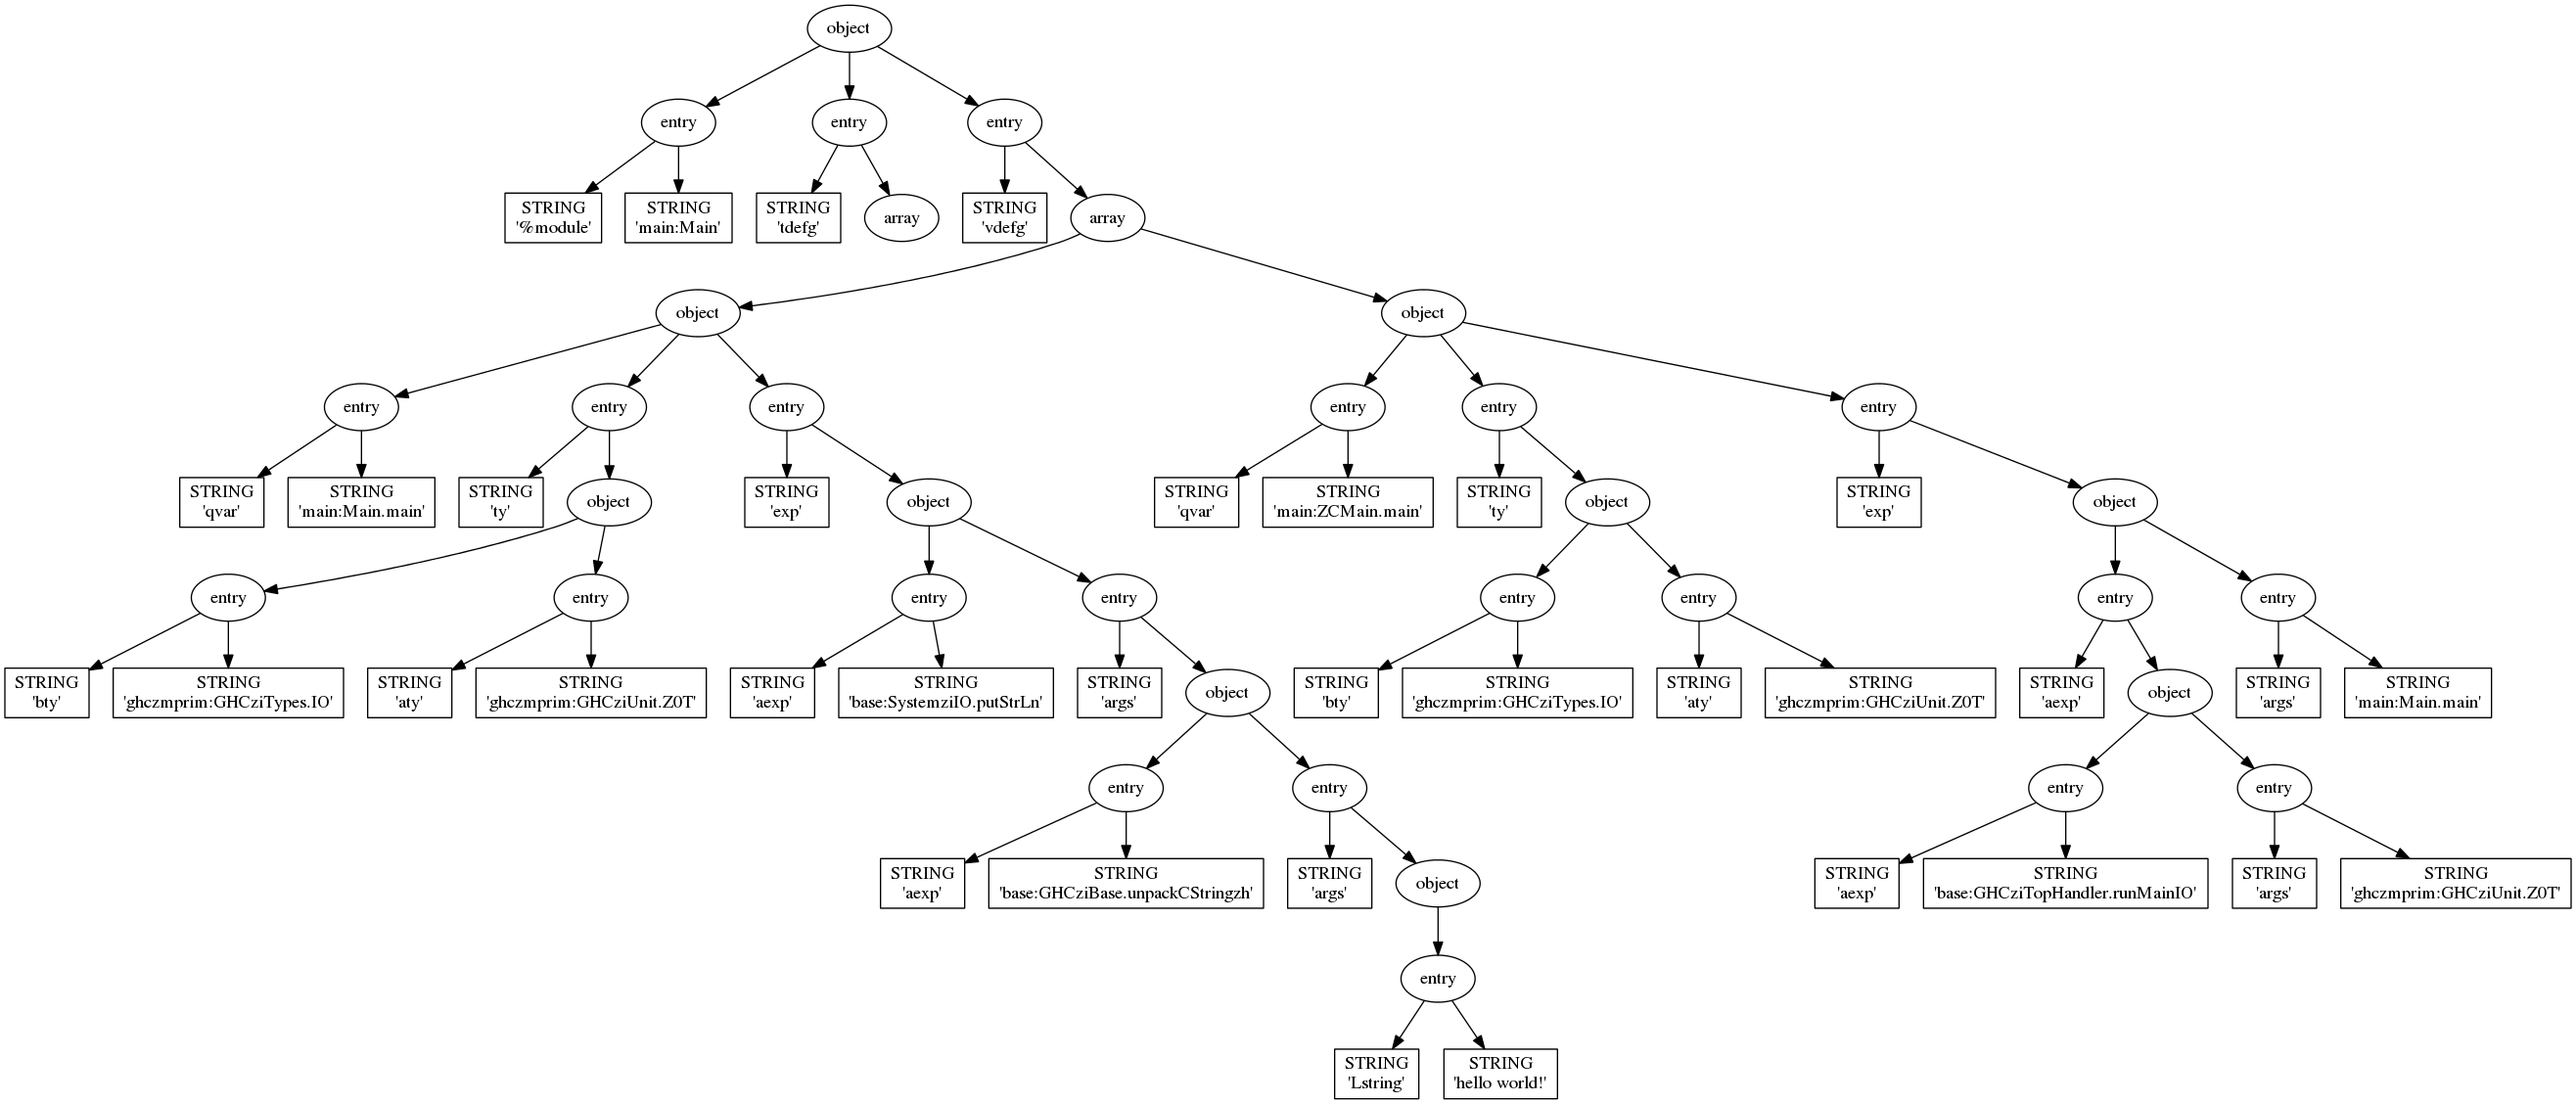
\includegraphics[width=\textwidth]{diags/helloworld2.png}
\caption{Example program translated to JSON}
\label{fig:helloworldgraph}
\end{figure}

\subsection{Compiler}

\subsubsection{Building the AST}




\bibliographystyle{plain}
\bibliography{papers}

\end{document}
